\documentclass[a4paper,12pt]{article} % добавить leqno в [] для нумерации слева
\usepackage[a4paper,top=1.3cm,bottom=2cm,left=1.5cm,right=1.5cm,marginparwidth=0.75cm]{geometry}
%%% Работа с русским языком
\usepackage{cmap}					% поиск в PDF
\usepackage{mathtext} 				% русские буквы в фомулах
\usepackage[T2A]{fontenc}			% кодировка
\usepackage[utf8]{inputenc}			% кодировка исходного текста
\usepackage[english,russian]{babel}	% локализация и переносы

\usepackage{graphicx}

\usepackage{wrapfig}
\usepackage{tabularx}

\usepackage{hyperref}
\usepackage[rgb]{xcolor}
\hypersetup{
colorlinks=true,urlcolor=blue
}
\usepackage{multirow}
\usepackage{hhline}


%%% Дополнительная работа с математикой
\usepackage{amsmath,amsfonts,amssymb,amsthm,mathtools} % AMS
\usepackage{icomma} % "Умная" запятая: $0,2$ --- число, $0, 2$ --- перечисление

%% Номера формул
\mathtoolsset{showonlyrefs=true} % Показывать номера только у тех формул, на которые есть \eqref{} в тексте.

%% Шрифты
\usepackage{euscript}	 % Шрифт Евклид
\usepackage{mathrsfs} % Красивый матшрифт

%% Свои команды
\DeclareMathOperator{\sgn}{\mathop{sgn}}

%% Перенос знаков в формулах (по Львовскому)
\newcommand*{\hm}[1]{#1\nobreak\discretionary{}
{\hbox{$\mathsurround=0pt #1$}}{}}

\begin{document}
	
	\begin{titlepage}
	\begin{center}
		{\large МОСКОВСКИЙ ФИЗИКО-ТЕХНИЧЕСКИЙ ИНСТИТУТ (НАЦИОНАЛЬНЫЙ ИССЛЕДОВАТЕЛЬСКИЙ УНИВЕРСИТЕТ)}
	\end{center}
	\begin{center}
		{\large Физтех-школа электроники, фотоники и молекулярной физики}
	\end{center}
	
	
	\vspace{4.5cm}
	{\huge
		\begin{center}
			{Лабораторные работы 4.6.1, 4.6.2}\\
			Интерференция электромагнитных волн миллиметрового диапазона. Туннелирование миллиметровых радиоволн
		\end{center}
	}
	\vspace{2cm}
	\begin{flushright}
		{\LARGE Салтыкова Дарья \\
			\vspace{0.5cm}
			Б04-105}
	\end{flushright}
	\vspace{8cm}
	\begin{center}
		Долгопрудный 2023
	\end{center}
\end{titlepage}

\section{Введение}

\noindent \textbf{Цель работы:}

\medskip

\noindent 4.6.1: Изучение интерференции электромагнитных волн миллиметрового диапазона с применением двух оптических интерференционных схем, экспериментальное определение длины волны излучения.

\medskip

\noindent 4.6.2: экспериментальное исследование эффекта проникновения электромагнитных волн — туннелирования — через воздушный зазор между диэлектрическими призмами при полном внутреннем отражении на границе диэлектрик-воздух.

\section{Экспериментальная установка 4.6.1}

\begin{figure}[h]
    \centering
    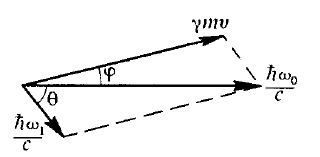
\includegraphics[width=12cm]{fig1.PNG}
    \caption{Приёмно-передающая система СВЧ-диапазона}
    \label{fig:vac}
\end{figure}

\noindent Применяемый в настоящей работе передатчик излучает линейно поляризованную волну, электрический вектор \textbf{E} которой перпендикулярен широкой стенке волновода. Приемник также может принимать только линейно поляризованную волну. Для установления связи в системе, изображенной на рис. 1, необходимо, чтобы широкие стенки волноводов передатчика и приемника были параллельны друг другу.

\medskip 

\noindent Если одну из антенн повернуть относительно луча на некоторый угол $\alpha$, интенсивность принимаемого сигнала будет изменяться по \textit{закону Малюса}
\begin{equation}
    I = I_0 \cos^2 \alpha
\end{equation}

\subsection{Интерференция радиоволн, отражённых от зеркала и решётки}

\begin{figure}[h]
    \centering
    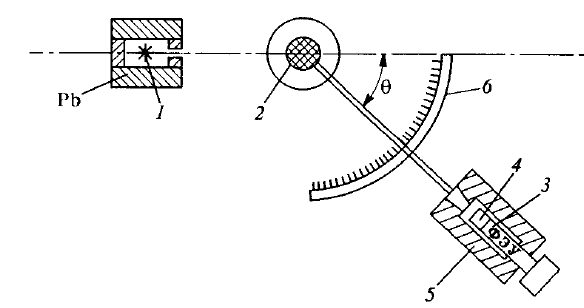
\includegraphics[width=6cm]{fig2.PNG}
    \caption{Интерференция волн СВЧ в плоскопараллельной пластине}
    \label{fig:vac}
\end{figure}

\noindent Между волнами, отраженными от решетки и от зеркала, возникает разность хода, равная
\begin{equation}
    \triangle = 2 d \cos \theta.
\end{equation}


\section{Ход работы 4.6.1}

\noindent 1. Закрепим на фиксаторах перед зеркалом металлическую решётку, убедимся, что при перемещении зеркала уровень сигнала в точке приёма изменяется.

\medskip

\noindent 2. Снимем зависимость интенсивности $I$ от координаты $x$ подвижного зеркала. Построим график зависимости $I(x)$
    
\begin{figure}[h]
    \centering
    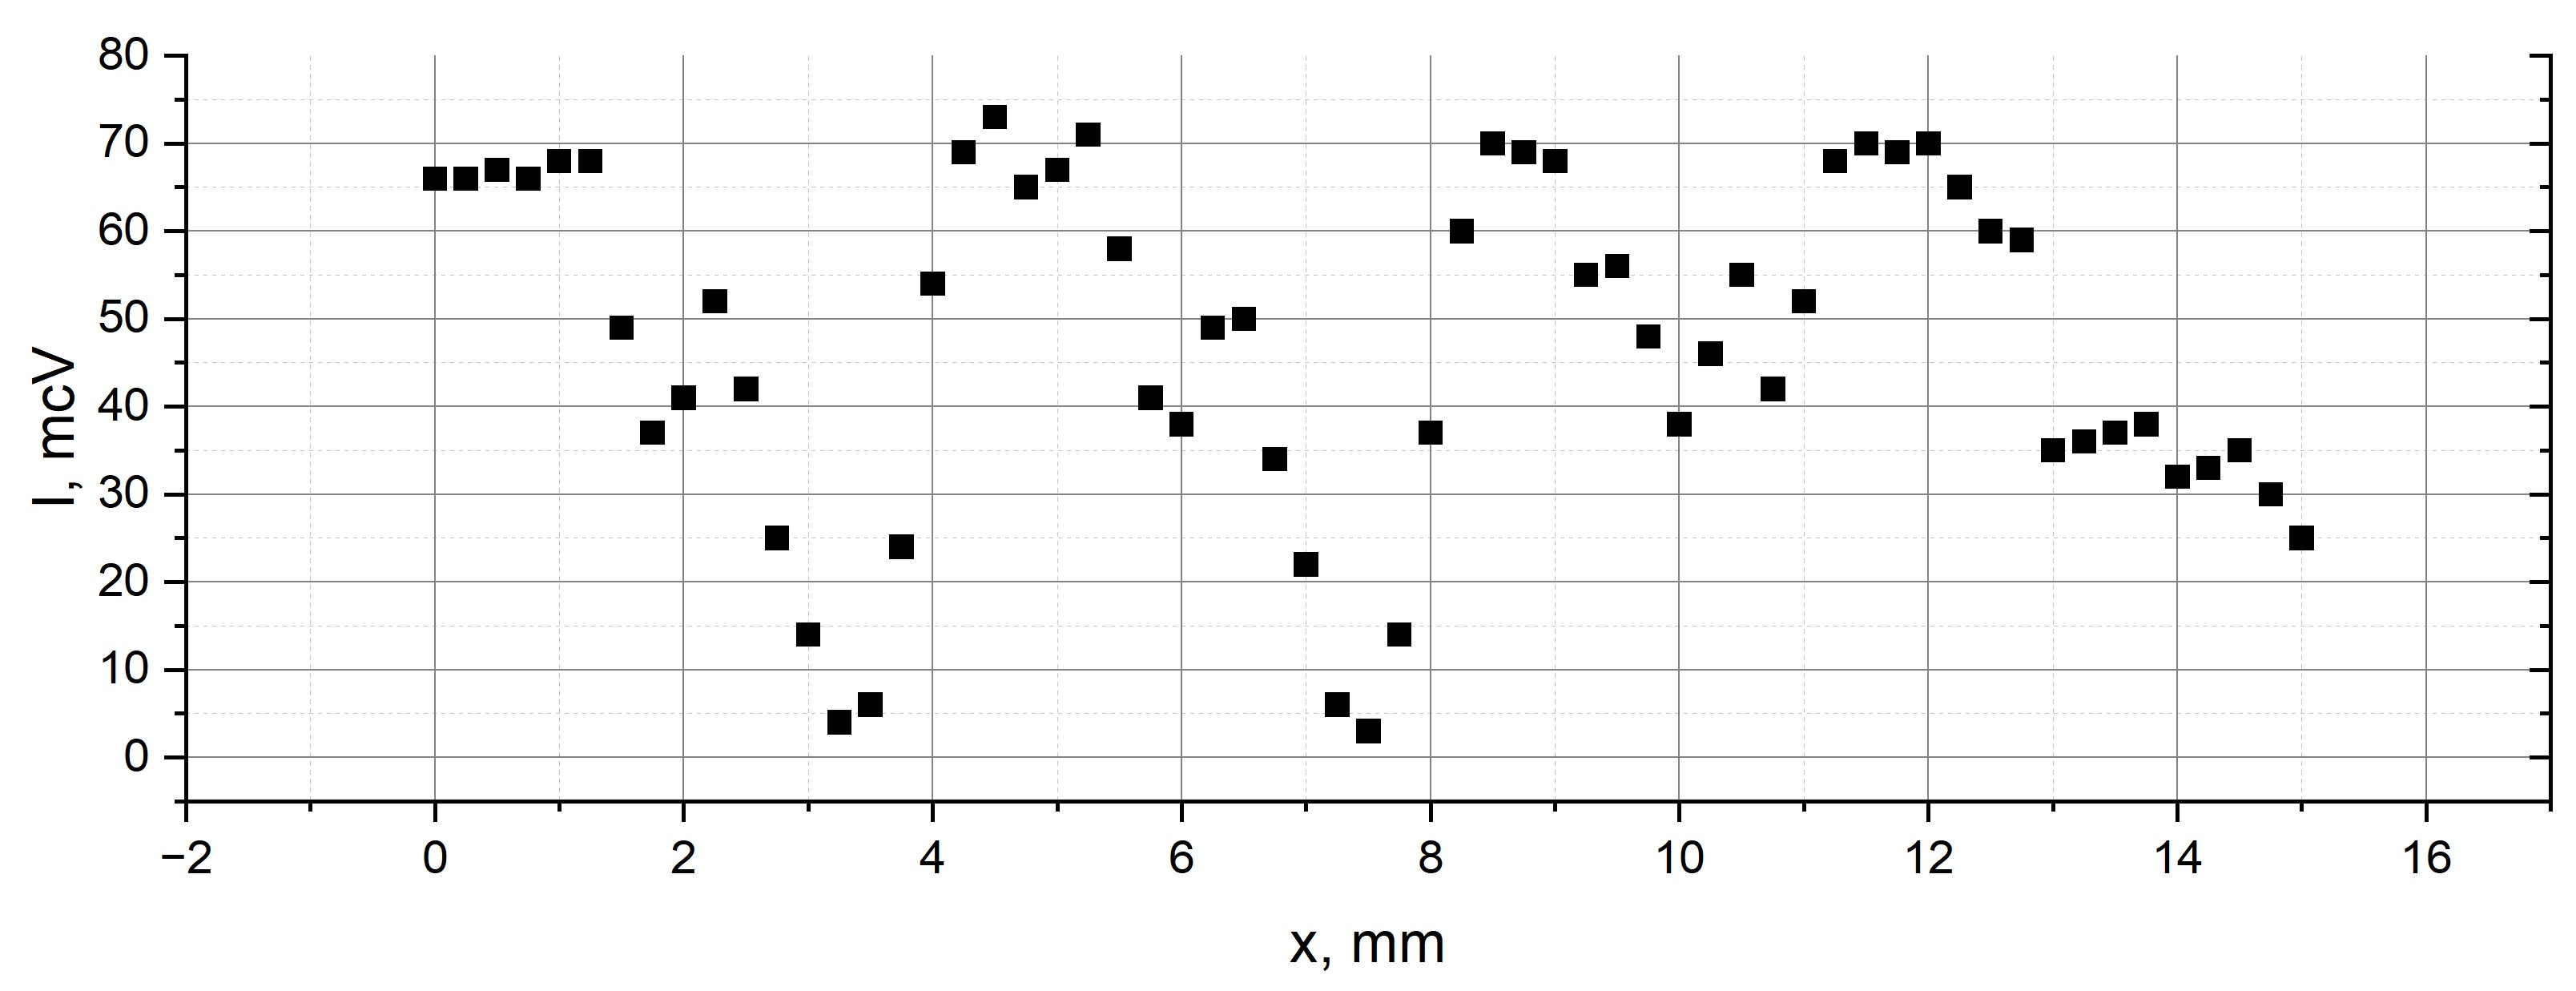
\includegraphics[width=14cm]{graph1.PNG}
    \caption{График зависимости интенсивности сигнала от координаты подвижного зеркала}
    \label{fig:vac}
\end{figure}

\noindent Длина волны, определённая по графику: $\lambda_\text{гр} = (8.3 \pm 0,1 )$ мм. \par

\medskip

\noindent Длина волны по частоте: $\lambda_\text{част} = 8.174$ мм ($\nu = $ 36,7 ГГЦ).

\section{Экспериментальная установка 4.6.2}

\noindent Генерирующий при выбранной настройке клистрон возбуждает в прямоугольном металлическом волноводе сечением 7,2 x 3,4 $\text{мм}^2$ электромагнитную волну, которая распространяется вдоль волновода и с помощью рупорной антенны $A_1$ излучается в пространство. Задача антенны заключается в том, чтобы сделать излучение более направленным. Электрический вектор волны, бегущей вдоль волновода и излучаемый антенной, перпендикулярен широкой стенке волновода. На пути радиоволн устанавливаются две одинаковые прямые призмы $\text{П}_1$ и $\text{П}_2$ с почти прямоугольным равнобедренным треугольником в основании. Уменьшение угла при вершине треугольника на $16^\circ$ сделано для устранения обратных отражений. Призмы изготовлены из фторопласта, обладающего малыми потерями на высоких радиочастотах. Узкие грани призм ограничивают воздушную прослойку, ширина которой может изменяться с помощью микрометрических винтов $M_1$ и $M_2$.
\begin{figure}
\begin{center}
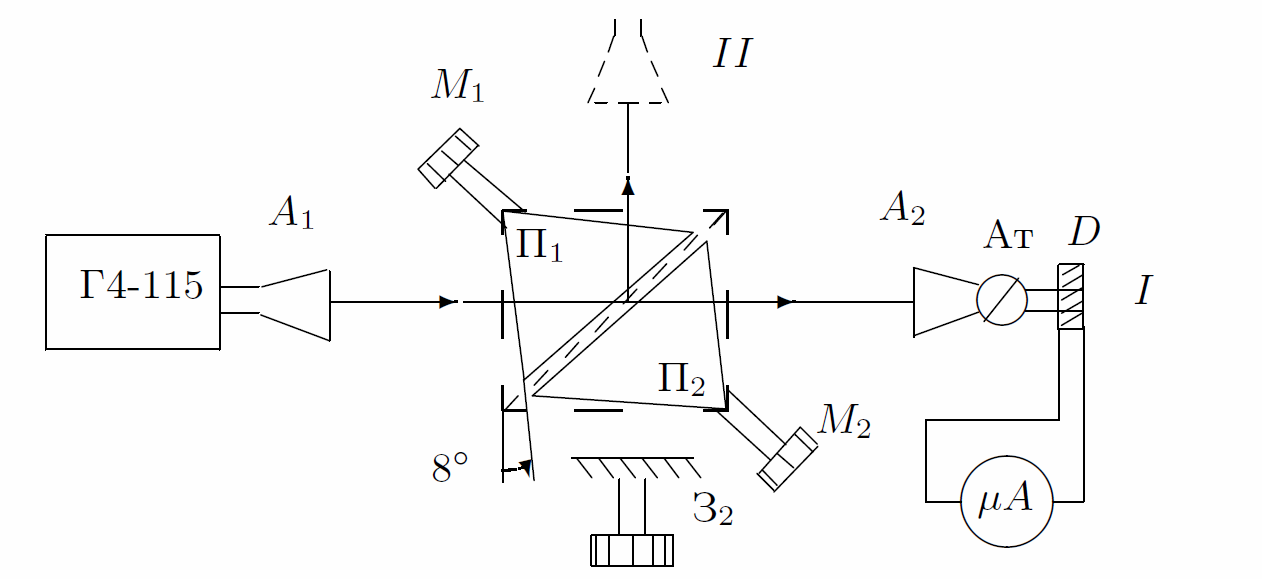
\includegraphics[width=0.5\textwidth]{tunnelteor}
\caption{Установка для исследования туннельного эффекта}
\end{center}

\end{figure}

\newpage

\section{Ход работы 4.6.2}

\noindent 1. Снимем зависимость интенсивности прошедшей волны от величины воздушного зазора. Результаты занесем в таблицу.\\
\medskip

\noindent 2. Переставим приёмник для измерения отраженного сигнала и снимем зависимость интенсивности отраженной волны от величины воздушного зазора.\\

\begin{table}[h!]
\begin{tabular}{|lll|lll|}
\hline
\multicolumn{3}{|l|}{$\text{пройденная}$}                                                        & \multicolumn{3}{l|}{$\text{отраженная}$}                                                      \\ \hline
\multicolumn{1}{|l|}{$z, \text{ мм}$} & \multicolumn{1}{l|}{$I_\text{пр},   \text{ мкА}$} & T    & \multicolumn{1}{l|}{$z, \text{ мм}$} & \multicolumn{1}{l|}{$I_\text{пр}, \text{ мкА}$} & R    \\ \hline
\multicolumn{1}{|l|}{0,00}            & \multicolumn{1}{l|}{100}                          & 1    & \multicolumn{1}{l|}{2,1}             & \multicolumn{1}{l|}{100}                        & 1    \\ \hline
\multicolumn{1}{|l|}{0,29}            & \multicolumn{1}{l|}{90}                           & 0,9  & \multicolumn{1}{l|}{1,92}            & \multicolumn{1}{l|}{89}                         & 0,89 \\ \hline
\multicolumn{1}{|l|}{0,54}            & \multicolumn{1}{l|}{80}                           & 0,8  & \multicolumn{1}{l|}{1,81}            & \multicolumn{1}{l|}{80}                         & 0,8  \\ \hline
\multicolumn{1}{|l|}{0,81}            & \multicolumn{1}{l|}{70}                           & 0,7  & \multicolumn{1}{l|}{1,49}            & \multicolumn{1}{l|}{70}                         & 0,7  \\ \hline
\multicolumn{1}{|l|}{1,16}            & \multicolumn{1}{l|}{60}                           & 0,6  & \multicolumn{1}{l|}{1,38}            & \multicolumn{1}{l|}{58}                         & 0,58 \\ \hline
\multicolumn{1}{|l|}{2,04}            & \multicolumn{1}{l|}{50}                           & 0,5  & \multicolumn{1}{l|}{1,06}            & \multicolumn{1}{l|}{50}                         & 0,5  \\ \hline
\multicolumn{1}{|l|}{2,69}            & \multicolumn{1}{l|}{40}                           & 0,4  & \multicolumn{1}{l|}{0,9}             & \multicolumn{1}{l|}{38}                         & 0,38 \\ \hline
\multicolumn{1}{|l|}{3,14}            & \multicolumn{1}{l|}{30}                           & 0,3  & \multicolumn{1}{l|}{0,57}            & \multicolumn{1}{l|}{30}                         & 0,3  \\ \hline
\multicolumn{1}{|l|}{3,62}            & \multicolumn{1}{l|}{20}                           & 0,2  & \multicolumn{1}{l|}{0,39}            & \multicolumn{1}{l|}{18}                         & 0,18 \\ \hline
\multicolumn{1}{|l|}{5,03}            & \multicolumn{1}{l|}{13}                           & 0,13 & \multicolumn{1}{l|}{0}               & \multicolumn{1}{l|}{13}                         & 0,13 \\ \hline
\end{tabular}
\end{table}


\noindent 3. Построим график зависимости коэффициентов T и R от величины воздушного зазора и убедимся, что T + R = 1.\\

\begin{figure}[!h]
\begin{center}
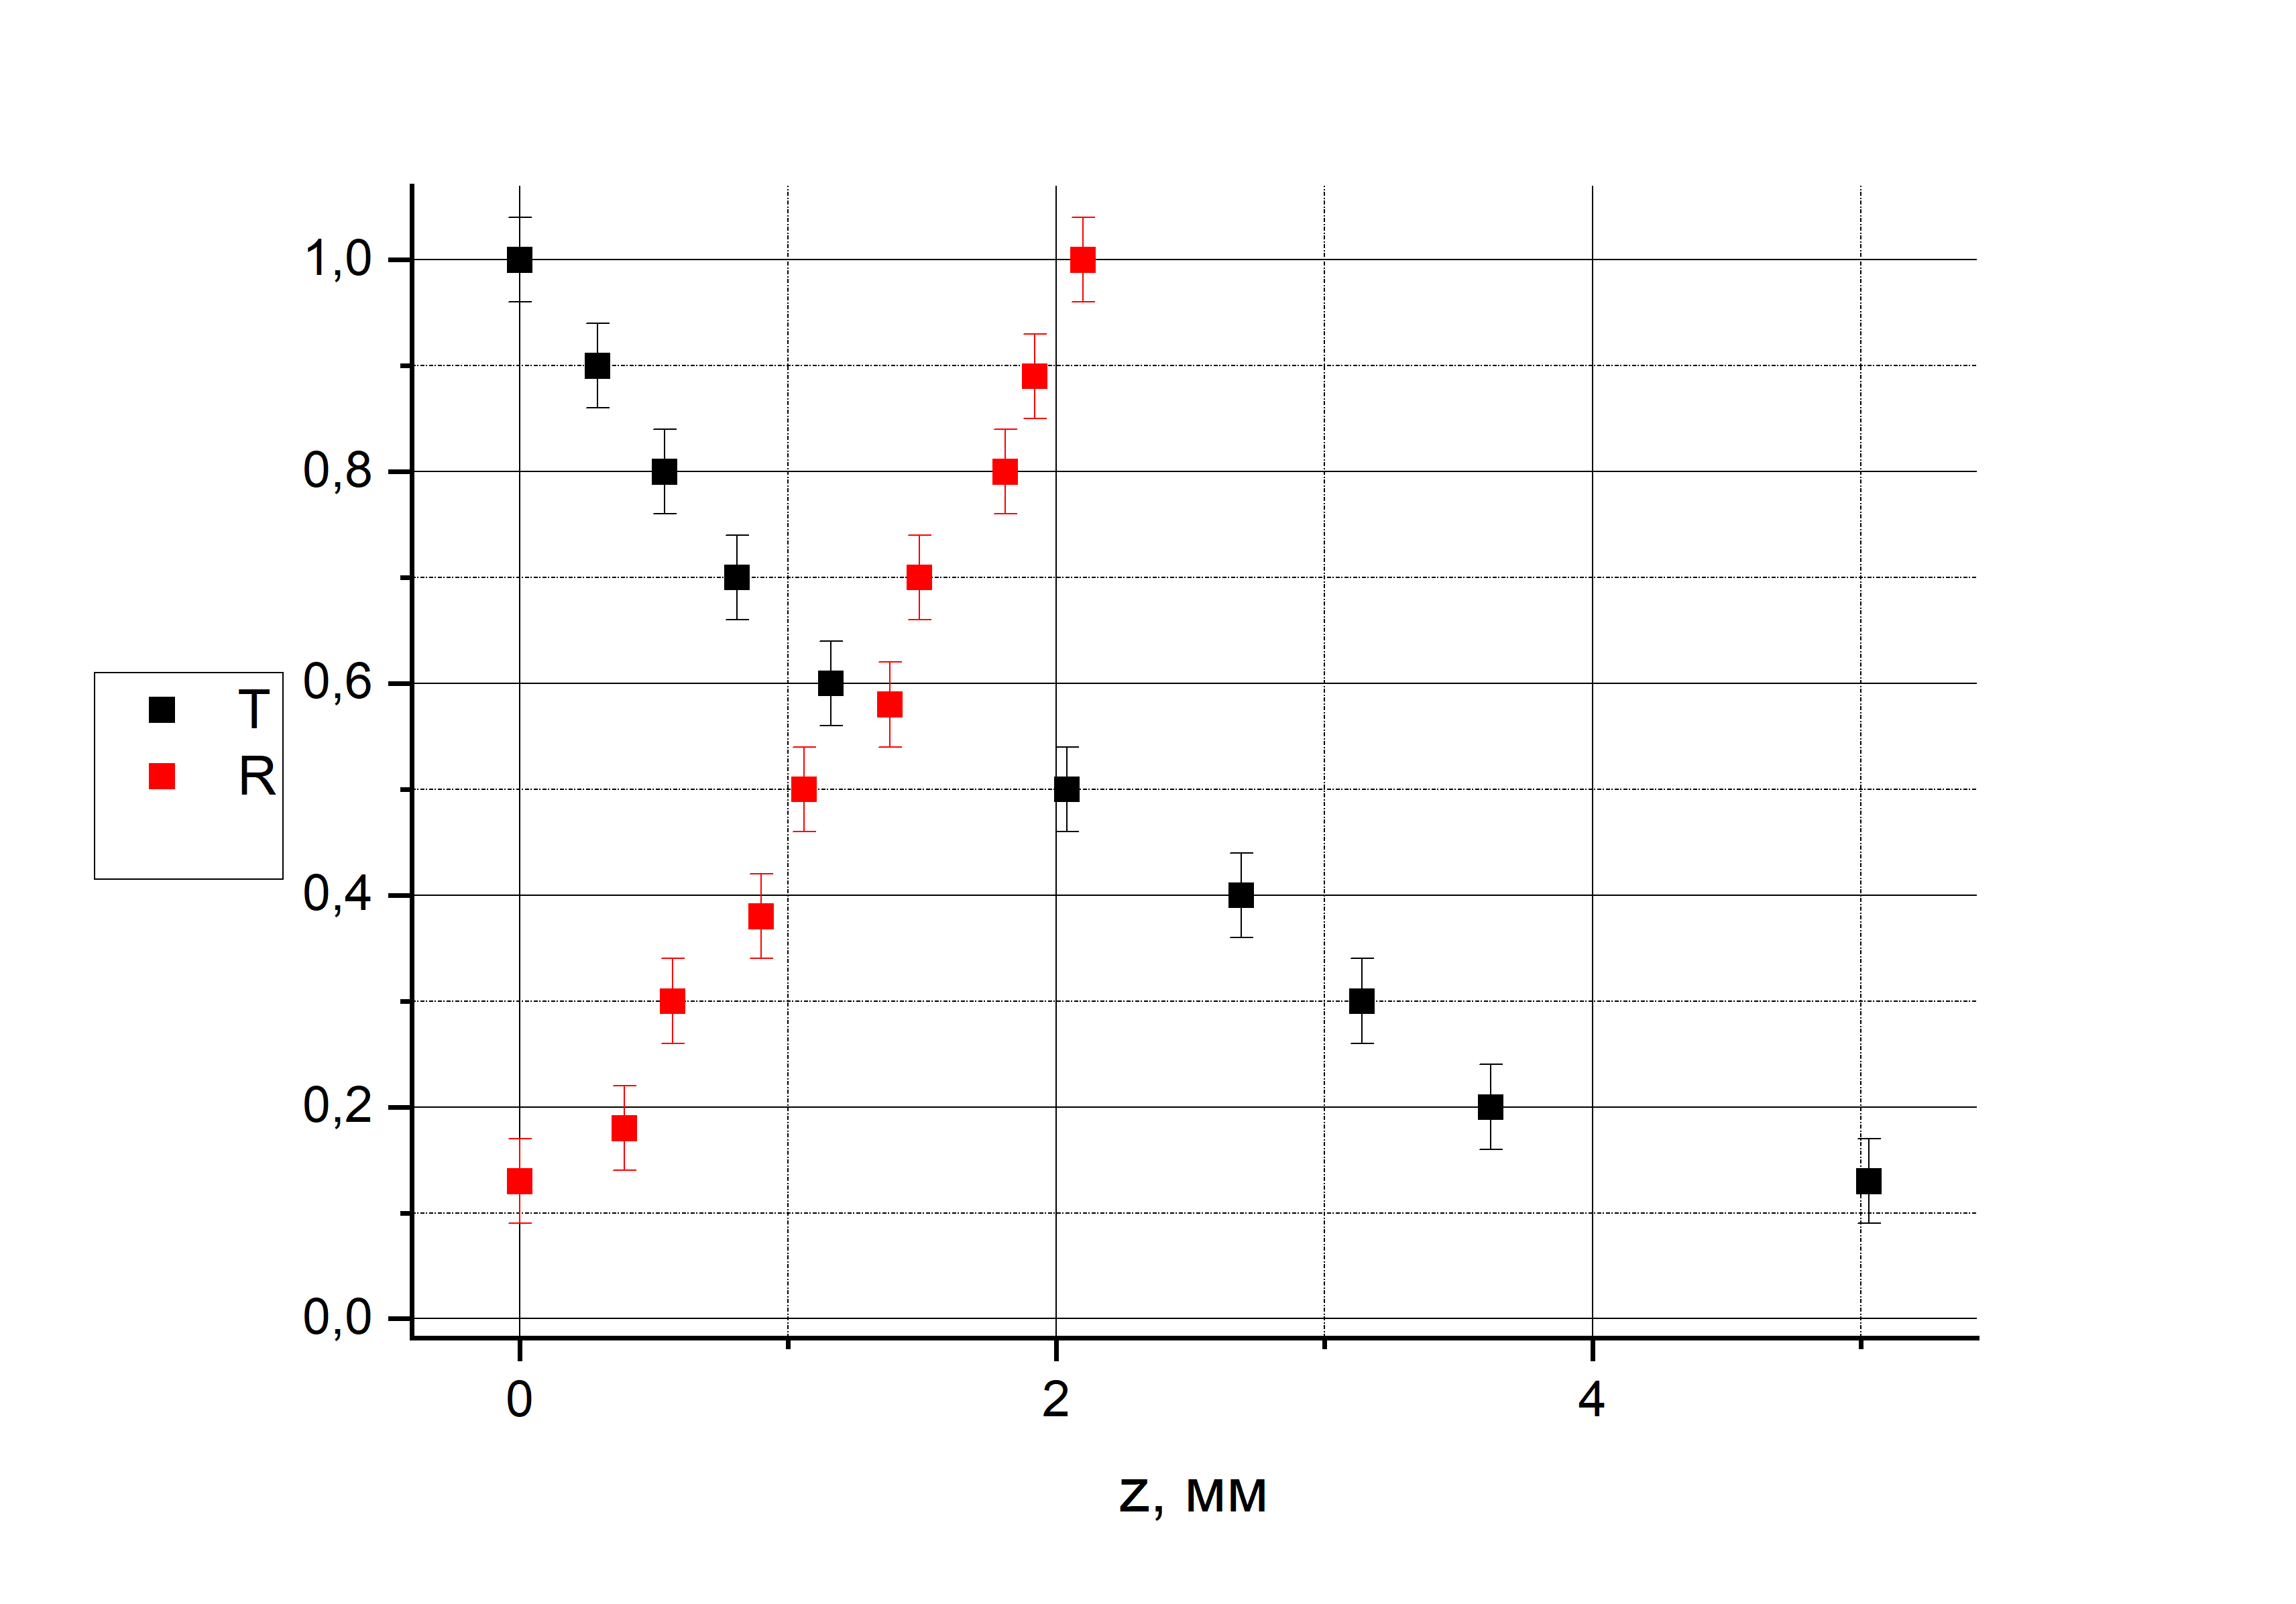
\includegraphics[width = 15cm]{graph2}
\end{center}
\end{figure}

\noindent 4. Построим график зависимости $ln(T)$ от показаний микрометра $z$.

\medskip

\begin{figure}[h!]
    \centering
    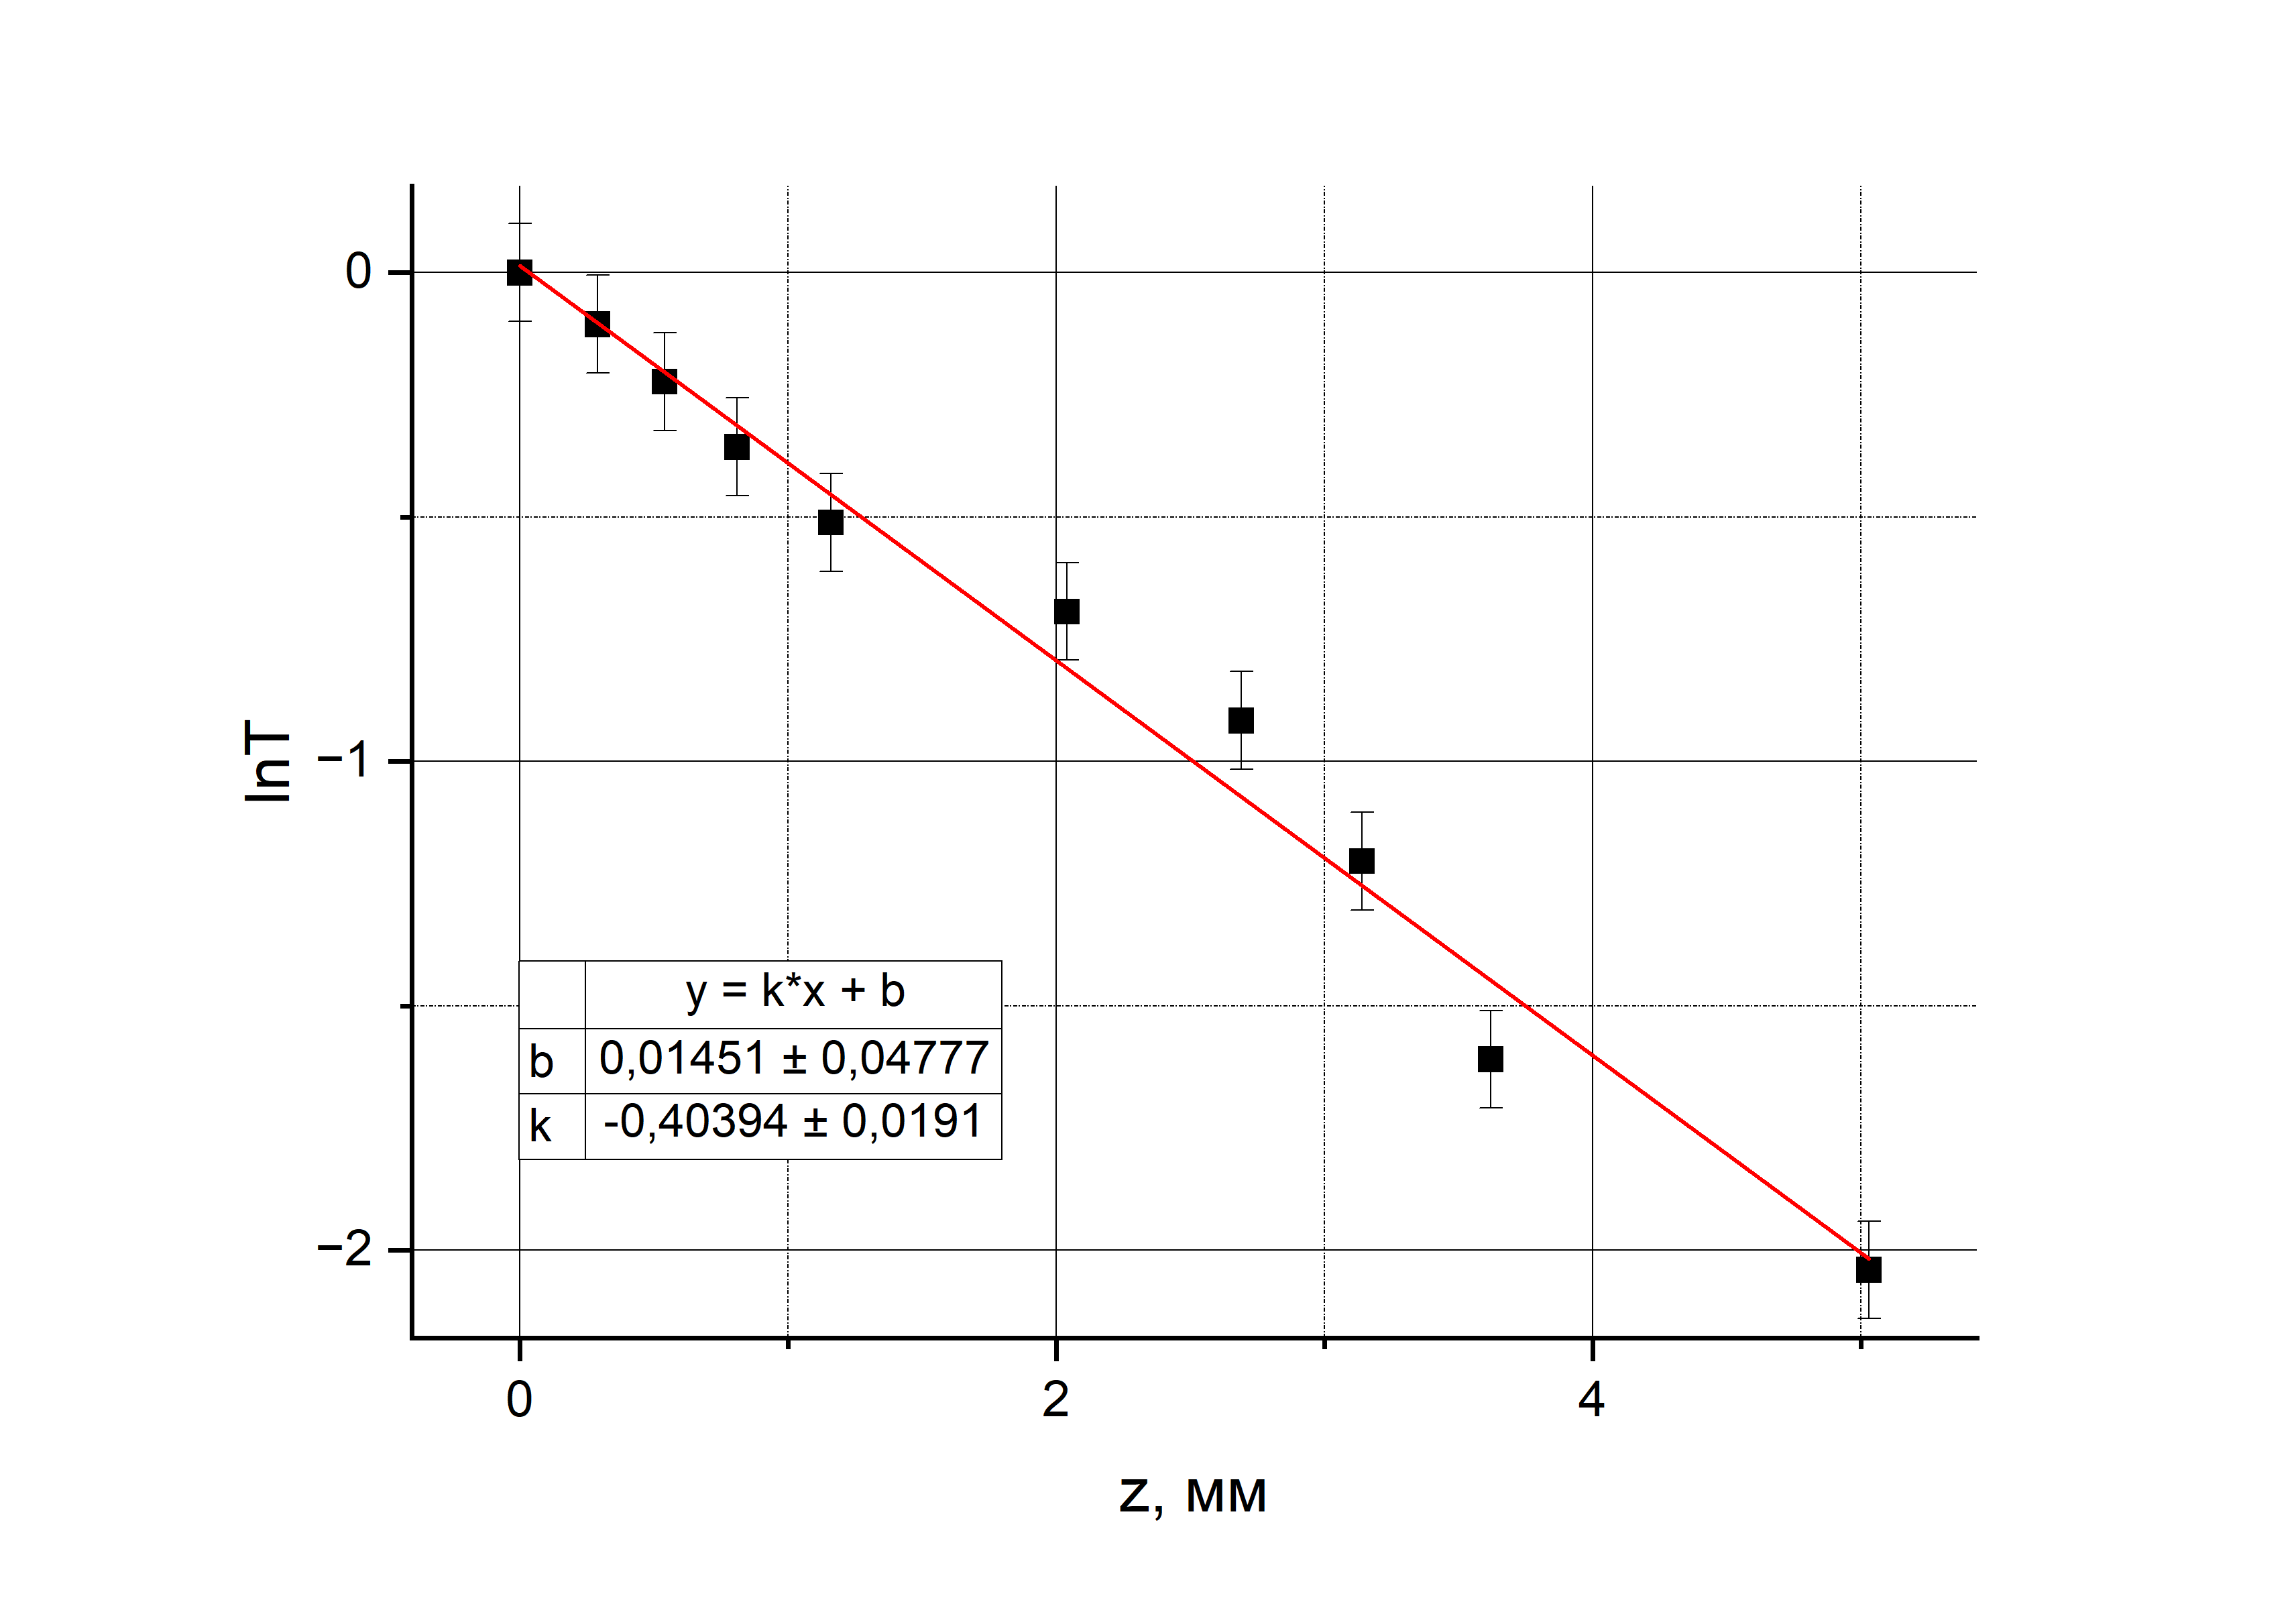
\includegraphics[width=16cm]{graph3.PNG}
    \caption{Зависимость $ln(T)$ от показаний $z$}
\end{figure}

\noindent Из наклона прямой получили значение длины затухания: $\Lambda = 2,5 \pm 0,1$ мм.

\medskip

\noindent Расчитаем показатель преломления фторопласта (частота генератора 36,5 ГГц): $n = 1,4 \pm 0,2$.\\

\section{Вывод}

\noindent В ходе работы:

\medskip

- Двумя способами определена длина волны, отраженной от зеркала и решетки. По графику: $\lambda_\text{гр} = (8.3 \pm 0,1 )$ мм, по частоте: $\lambda_\text{част} = 8.174$ мм.

\medskip

- При исследовании туннелирования радиоволн получено значение длины затухания: $\Lambda = (2,5 \pm 0,1)$ мм и рассчитан показатель преломления фторопласта: $n = 1,4 \pm 0,2$.

\end{document}